\documentclass[a4paper]{scrreprt}
\usepackage{etex}
\usepackage[utf8]{inputenc}
%\usepackage[T1]{fontenc}
\usepackage{lmodern}
\usepackage{hyphsubst}
\usepackage[english]{babel}
\usepackage{textcomp}
\usepackage{enumerate}
\usepackage{microtype}
\usepackage{listings}
\usepackage{graphicx}
\usepackage{subcaption}
\usepackage{titling}
\usepackage{amsmath}
\usepackage{float}
\lstset{language=[LaTeX]TeX}

\usepackage{wallpaper}

\renewcommand{\quote}[1]{``#1''}

\begin{document}
\URCornerWallPaper{0.25}{TUHH.png}
\title{Report on Exam Task\\Simulation and Modelling of Communication Networks}
\author{Nicolás Chopitea Kober, Sebastian Lindner}
\date{Summer Term 2016}
\maketitle	

\chapter{Overview}
\section{Requirement Analysis}
	\subsection{Network Description}
	\subsection{Statistical Web Browsing Model}
		The student's web browsing behavior is difficult to capture. We are going to model it by assuming a student issues an HTTP request, receives a response and then spends some time reading the response that is exponentially distributed. Missing at this point is the size of the response that follows a request. To model this we have analyzed a trace file containing 1000 response size values.
		
		We have chosen the \emph{chi squared goodness of fit test} to evaluate how well a distribution fits the observed data. As a first step we investigated the density of values within intervals that initially were of equal size and then potentially merged to remove those that contained no observed value. In this way 250 initially equal-sized intervals were reduced to 160 of which most have observed values associated to them. This is a graphical representation of what we found:
		\begin{figure}[H]
		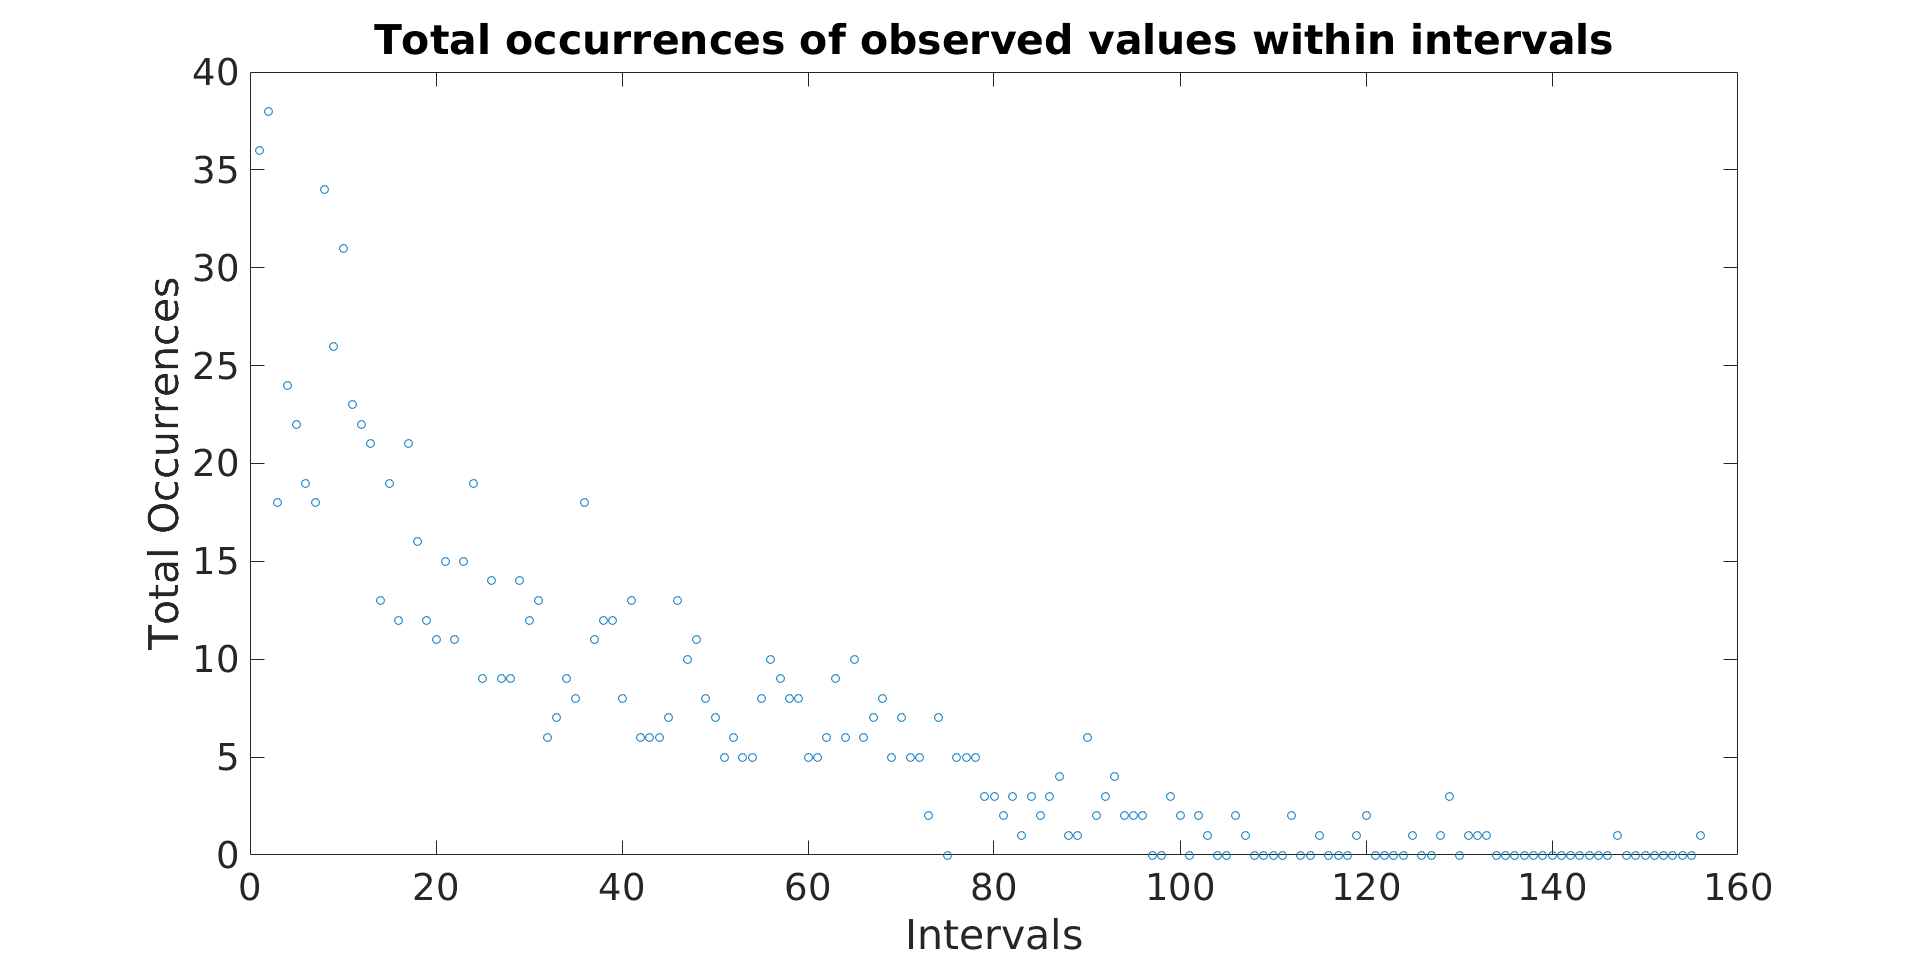
\includegraphics[width=\textwidth]{../tracefile_analysis/exp.png}
		\caption{Request size value density in intervals}
		\end{figure}
		
		We have the highest density of observed values in regions of low response sizes, and the number of observations decreases for increasing response sizes. This looks closely related to values coming from a \emph{negative exponential distribution}, which is why we decided to apply the test against this distribution.
		
		The test states that the observed values follow an Exponential distribution with mean $\lambda=580390\,\text{Byte}$ at a significance level of $99.95\%$.
		
		

\end{document}
